\documentclass[tikz,border=4pt]{standalone}
% Shared visual grammar: role fills, dark connectors, and 7-point typography.
% Build each standalone figure from this directory. No external images required.
\pdfinfoomitdate=1
\pdftrailerid{}
\usepackage[T1]{fontenc}
\usepackage{helvet}
\renewcommand{\familydefault}{\sfdefault}
\usepackage{amsmath,amssymb}
\hyphenpenalty=10000
\exhyphenpenalty=10000
\usetikzlibrary{arrows.meta,calc,fit,positioning,decorations.pathreplacing,backgrounds}
\definecolor{ink}{HTML}{172B3A}
\definecolor{muted}{HTML}{586D85}
\definecolor{datafill}{HTML}{F1F5F9}
\definecolor{dataline}{HTML}{62748E}
\definecolor{modelfill}{HTML}{E5E9FF}
\definecolor{modelline}{HTML}{7887C7}
\definecolor{llmfill}{HTML}{FFE4E8}
\definecolor{llmline}{HTML}{E68494}
\definecolor{truthfill}{HTML}{D0FAE5}
\definecolor{truthline}{HTML}{35A782}
\newcommand{\seven}{\fontsize{7}{8.5}\selectfont}
\tikzset{
 every node/.append style={font=\seven,text=ink,align=center},
 box/.style={draw=dataline,fill=white,rounded corners=3pt,line width=.65pt,inner sep=5pt,minimum height=8mm},
 data/.style={box,fill=datafill},
 model/.style={box,draw=modelline,fill=modelfill},
 llm/.style={box,draw=llmline,fill=llmfill},
 truth/.style={box,draw=truthline,fill=truthfill},
 title/.style={font=\seven\bfseries,inner sep=1pt},
 word/.style={text=muted,inner sep=1pt,align=center},
 label/.style={fill=white,inner xsep=2pt,inner ysep=1pt,text=muted},
 flow/.style={-{Stealth[length=2.4mm,width=1.9mm]},draw=ink,line width=1.2pt,shorten >=1.5pt},
 branch/.style={-{Stealth[length=2mm,width=1.6mm]},draw=ink,line width=.9pt,shorten >=1pt},
 route/.style={draw=ink,line width=1.2pt},
 update/.style={-{Stealth[length=2.2mm,width=1.7mm]},draw=modelline,line width=1pt,dash pattern=on 3pt off 2pt,shorten >=1.5pt},
 boundary/.style={draw=dataline,dash pattern=on 3pt off 2pt,rounded corners=3pt,line width=.6pt},
 chip/.style={minimum height=4mm,inner xsep=3pt,inner ysep=1.5pt,rounded corners=2pt},
}
% Optional role key. Anchor at the center of an uncluttered final row.
\newcommand{\rolekey}[2]{
 \node[word,anchor=east] at (#1-6.6,#2) {\textit{Key}};
 \node[data,chip] at (#1-5.2,#2) {records / data};
 \node[model,chip] at (#1-1.9,#2) {learned model / policy};
 \node[llm,chip] at (#1+1.65,#2) {LLM signal};
 \node[truth,chip] at (#1+4.95,#2) {labels / evaluation};
}

\begin{document}
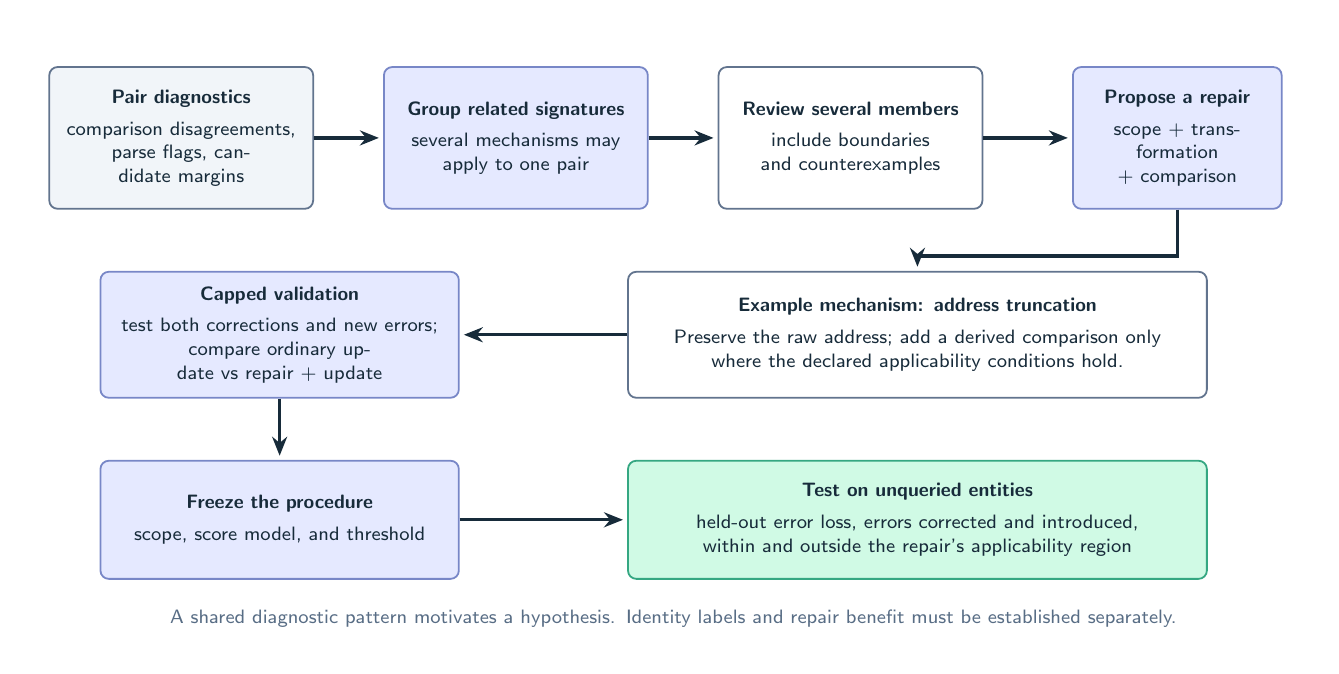
\begin{tikzpicture}

\useasboundingbox (-.2,.3) rectangle (16.1,-7.55);
\node[data,text width=30mm,minimum height=18mm] (diag) at (1.75,-1.1) {\textbf{Pair diagnostics}\\[3pt]comparison disagreements,\\parse flags, candidate margins};
\node[model,text width=30mm,minimum height=18mm] (group) at (6,-1.1) {\textbf{Group related signatures}\\[3pt]several mechanisms may\\apply to one pair};
\node[box,text width=30mm,minimum height=18mm] (review) at (10.25,-1.1) {\textbf{Review several members}\\[3pt]include boundaries\\and counterexamples};
\node[model,text width=23mm,minimum height=18mm] (repair) at (14.4,-1.1) {\textbf{Propose a repair}\\[3pt]scope + transformation\\+ comparison};
\draw[flow] (diag) -- (group); \draw[flow] (group) -- (review); \draw[flow] (review) -- (repair);
\node[box,text width=70mm,minimum height=16mm] (spec) at (11.1,-3.6) {\textbf{Example mechanism: address truncation}\\[3pt]Preserve the raw address; add a derived comparison only\\where the declared applicability conditions hold.};
\draw[flow] (repair.south) -- (14.4,-2.6) -| (spec.north);
\node[model,text width=42mm,minimum height=16mm] (validate) at (3,-3.6) {\textbf{Capped validation}\\[3pt]test both corrections and new errors;\\compare ordinary update vs repair + update};
\draw[flow] (spec.west) -- (validate.east);
\node[model,text width=42mm,minimum height=15mm] (freeze) at (3,-5.95) {\textbf{Freeze the procedure}\\[3pt]scope, score model, and threshold};
\node[truth,text width=70mm,minimum height=15mm] (test) at (11.1,-5.95) {\textbf{Test on unqueried entities}\\[3pt]held-out error loss, errors corrected and introduced,\\within and outside the repair's applicability region};
\draw[flow] (validate) -- (freeze); \draw[flow] (freeze) -- (test);
\node[word,text width=143mm] at (8,-7.2) {A shared diagnostic pattern motivates a hypothesis. Identity labels and repair benefit must be established separately.};

\end{tikzpicture}
\end{document}
